\documentclass[11pt,a4paper]{article}
\usepackage[margin=2.1cm]{geometry}
\usepackage{amsmath,booktabs,tabularx,xcolor,hyperref,enumitem,graphicx,float,longtable}
\hypersetup{colorlinks,linkcolor=blue!50!black,urlcolor=blue!50!black}
\setlist{itemsep=1pt,topsep=2pt}
\newcommand{\code}[1]{\texttt{\small #1}}
\definecolor{bad}{HTML}{B5403A}\definecolor{good}{HTML}{2E7D4F}

\title{Did the Wolfe Trahan relationships predict company results?\\[2pt]\large A firm-level test of eight 2011 claims on US non-financial companies, 1994--2026}
\author{FundamentalQuantmental, HY Analyst}
\date{Run 24 October 2026. Decision page: \code{docs/decisions/2026-10-24-wt-relationship-tests.md}}

\begin{document}
\maketitle

\noindent\fcolorbox{gray}{gray!6}{\parbox{\dimexpr\linewidth-2\fboxsep-2\fboxrule}{%
\textbf{The answer}
\begin{enumerate}
\item \textbf{\color{bad}Mostly no.} We ran 92 tests on 17,767 companies (87 had enough data for every statistic). Only 3 passed every rule we set in advance. After the robustness checks (Section~\ref{sec:robust}), none is robust.
\item \textbf{One small effect survives the strictest test, but it is fragile.} When factory input prices jump, the costs of highly leveraged industrial companies rise by about 0.2\% of sales within two quarters. It is the only test that survives a correction across all 92 tests (Romano--Wolf $p$ = 0.024). It holds only when every company counts equally, and it disappears when companies are weighted by sales. So it is a small-company effect.
\item \textbf{\color{bad}The sales claim was backwards.} The notes say input-price jumps come before slower sales. In fact, sales sped up after a jump ($t = +5.2$ after 2011). The jumps came at the start of recoveries.
\item \textbf{\color{good}Two directions hold, but they do not improve forecasts.} High inflation went with weaker consumer EBITDA and margins. Rising oil went with higher energy EBITDA and higher consumer costs. Both held the claimed way in both periods. Neither added enough to a forecast to pass.
\item \textbf{\color{bad}Two of the model's own macro inputs failed after 2011.} Bank lending standards and the factory survey did not predict company EBITDA declines after 2011. The Baa spread did a little.
\item \textbf{\color{good}Company sensitivities persist for some signals.} Companies that reacted more to input prices or to the Korean stock market in the past reacted more again. This supports a sensitivity per issuer, not one per sector.
\end{enumerate}
\textbf{What to do.} Add none of these series to the model's forecast inputs. Use the confirmed directions (H2, H3) only to set signs in the stress scenarios. Open a decision page to review the macro inputs of the downside model (methodology 5.2).}}

\section*{The question}
Each claim says: when a macro series moves, the companies in a sector later report different numbers. We asked whether that happened in history, company by company. A claim is useful only if it predicts \emph{company} results. Those results drive leverage, interest cover, and default risk.

\section{What we tested}
The 2011 notes chart pairs of series. We kept the eight claims that map to company results (decision page, ``The eight claims to test''). The sign and the lead of each claim come from the note. We did not search over leads.

\begin{center}\small
\begin{tabularx}{\linewidth}{@{}l>{\raggedright}p{3.3cm}X@{}}\toprule
Claim & Signal & Claimed effect on companies \\\midrule
H1 & Factory prices paid (Philadelphia Fed) & Costs rise within 2 quarters; sales slow within 4 quarters. Industrials, materials, consumer \\
H1c & H1, 6-month jump instead of level & Same as H1. A cross-check: the first run used this signal \\
H2 & CPI inflation, year on year & Consumer EBITDA and margin fall; energy and materials EBITDA rise \\
H3 & Oil price, year on year & Energy EBITDA rises; costs of transport and consumer companies rise \\
H4 & Housing starts, year on year & Homebuilders' and building-product makers' EBITDA and sales rise \\
H5, H5k & Copper; Korean stock market (KOSPI) & Sales of materials and industrial companies speed up within 2 quarters \\
H6 & Factory new orders (Philadelphia Fed) & Sales and EBITDA of industrials, materials, autos rise \\
H7, H7n & Real yield curve (10-year minus CPI); nominal curve (10-year minus 3-month) & A steeper curve means fewer large EBITDA declines a year ahead \\
H8a--c & Baa spread change; bank lending standards; factory activity & The model's current inputs: more (fewer) large EBITDA declines a year ahead \\\bottomrule
\end{tabularx}
\end{center}

\section{Data and method}
\begin{enumerate}
\item \textbf{Companies.} Compustat quarterly, all US non-financial companies (every GICS sector except financials and real estate), 1992--2026. A company enters a quarter when its sales over the last four quarters exceed \$40m. That gives 17,767 companies and 446,255 company-quarters. Each company counts once. So the test reflects the typical company, not the largest ones.
\item \textbf{Outcomes, per company.} All measures use four-quarter totals, which removes seasonal swings. All measures cover the quarters \emph{after} the signal quarter:
cost ratio (cost of goods sold over sales), change over 2 quarters; EBITDA margin, change over 4 quarters; EBITDA change over 4 quarters, as a share of sales; sales growth, next 4 (or 2) quarters minus the previous 4 (or 2); leverage (debt over EBITDA); and a large-decline event, EBITDA down by more than 20\% in 4 quarters. Extreme values are trimmed at 1\% and 99\% each quarter.
\item \textbf{Signals, as known then.} Each macro value enters only when published. CPI and housing starts enter one month late. Each signal is a $z$-score against its own history up to that quarter.
\item \textbf{High-leverage companies.} Debt above 4 times EBITDA. These are the companies closest to high-yield issuers.
\item \textbf{Three tests.}
\begin{itemize}
\item \textbf{A: the average company in the group.} The equal-weighted mean outcome each quarter. Run on all companies, and on high-leverage companies only.
\item \textbf{B: the group against a comparison group, in the same quarter.} For example, consumer companies minus energy and materials companies. The common economic swing drops out. This equals a company panel with a fixed effect for each quarter.
\item \textbf{C: each company's own sensitivity.} Each quarter, estimate how much each company reacted to the signal in its own past. Then ask whether those that reacted more before react more again (Fama--MacBeth). A slope of 1 means full carry-over. A slope of 0 means none.
\end{itemize}
\item \textbf{Statistics for A and B.} The study runs a regression of the outcome on the signal. The controls are factory activity, the Baa spread change, bank lending standards, and the outcome's own recent past. Newey--West errors correct for the overlapping horizons. The study runs the regression on 1994--2011 (the years the notes could see) and on 2012--2026 (the true test). A forecast race from 2012 compares a model with the signal against the model without it (Clark--West). The study also counts the signal episodes and checks the four cycle windows (2008--09, 2015--16, 2020, 2022).
\item \textbf{Pass rule (set in advance).} Right sign after 2011. A forecast gain with $p < 0.05/8$. The claimed sign in at least 3 of the 4 cycles, and in at least 2 of the 3 after 2011.
\end{enumerate}

\section{Results}
\begin{figure}[H]\centering
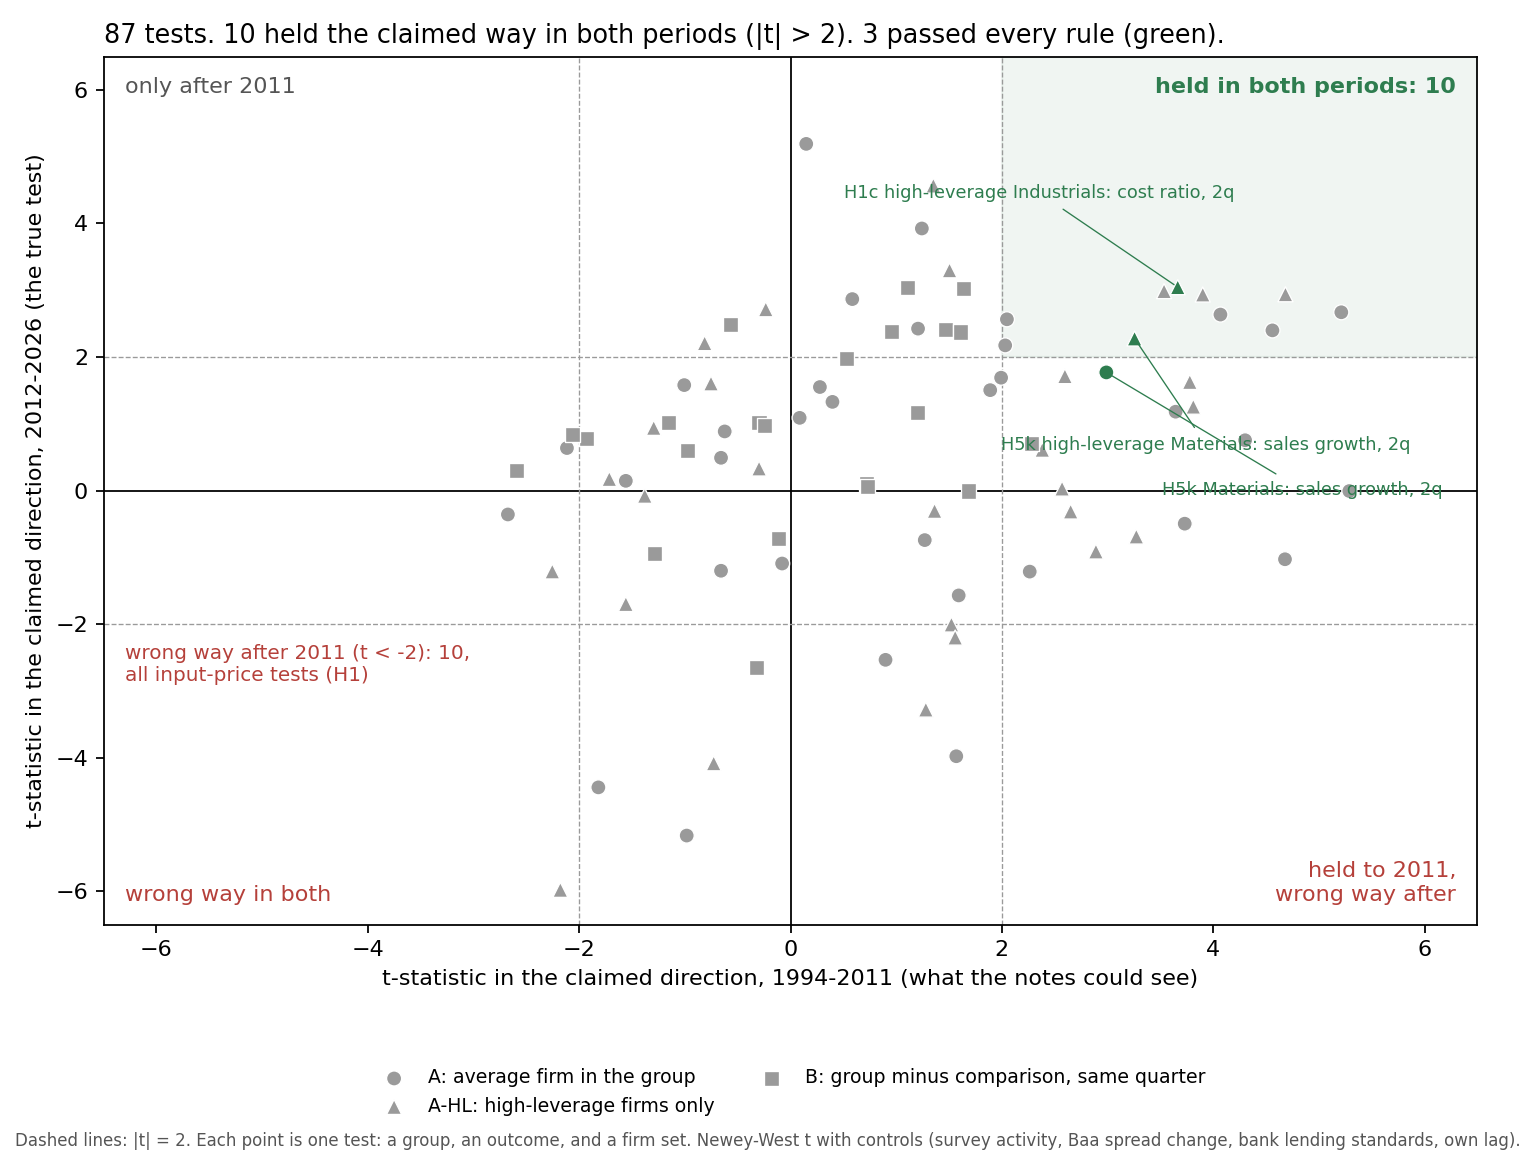
\includegraphics[width=0.93\linewidth]{figures/wt_scorecard.png}
\caption{Each point is one test. The horizontal axis shows the evidence in the years the notes could see. The vertical axis shows the evidence after 2011. A useful claim sits top right. Ten tests sit there. Ten tests went clearly the wrong way after 2011, and all ten are input-price tests.}
\end{figure}

\subsection*{Claim by claim}
\begin{center}\small
\begin{tabularx}{\linewidth}{@{}l>{\raggedright}p{2.2cm}X@{}}\toprule
Claim & Verdict & Evidence \\\midrule
H1 & \color{bad}Failed & Costs of the average industrial and consumer company rose after high prices paid to 2011 ($t$ +4.7, +4.3). After 2011 the effect is near zero. The sales claim fails. 0 of 18 tests pass. \\
H1c & \color{good}One pass & High-leverage industrials: costs up 0.22 points of sales per 1 sd jump, within 2 quarters ($t$ +3.7 to 2011, +3.1 after; forecast gain $p$ = 0.0001; 3 of 4 cycles). Sales sped up instead of slowing ($t$ +3.3 to +6.0 against the claim, after 2011). \\
H2 & \color{good}Direction holds & Consumer EBITDA fell with high inflation ($t$ $-5.2$ to 2011, $-2.7$ after). Margin too ($-4.6$, $-2.4$). 3 of 4 cycles. No forecast gain ($p$ = 0.12, 0.09). The commodity side and the consumer-minus-commodity test fail. \\
H3 & \color{good}Direction holds & Energy EBITDA rose with oil, strongest for high-leverage energy companies after 2011 ($t$ +4.6; $p$ = 0.014). Consumer costs rose ($t$ +4.1, +2.6; $p$ = 0.036). Transport fails. \\
H4 & \color{bad}Failed & Housing-linked EBITDA followed housing starts only after 2011 ($t$ +0.2 to 2011, +5.2 after). About 55 companies a quarter. \\
H5 & \color{bad}Failed & Copper did not predict sales. \\
H5k & \color{good}Passes the rule & Materials sales sped up 2.8 points per 1 sd of KOSPI growth, within 2 quarters ($t$ +3.0 to 2011, +1.8 after; $p$ = 0.006; high leverage $p$ = 0.0006). Just misses the strictest correction. \\
H6 & \color{bad}Failed & New orders predicted neither sales nor EBITDA, for any group. \\
H7 & \color{bad}Failed & A steep real curve went with fewer declines after 2011 ($t$ $-3.9$) but not before ($-1.2$). No forecast gain. The nominal curve fails too. \\
H8a & Weak & A wider Baa spread went with more declines. For high-leverage companies $t$ is +3.5 to 2011 and +3.0 after ($p$ = 0.04). For all companies, 4 of 4 cycles ($p$ = 0.016). Closest of the model's inputs. \\
H8b & \color{bad}Failed after 2011 & Bank lending standards: $t$ +5.3 to 2011, 0.0 after. \\
H8c & \color{bad}Failed & Factory activity: no relation in either period. \\\bottomrule
\end{tabularx}
\end{center}

\subsection*{Why the input-price claim failed}
\begin{figure}[H]\centering
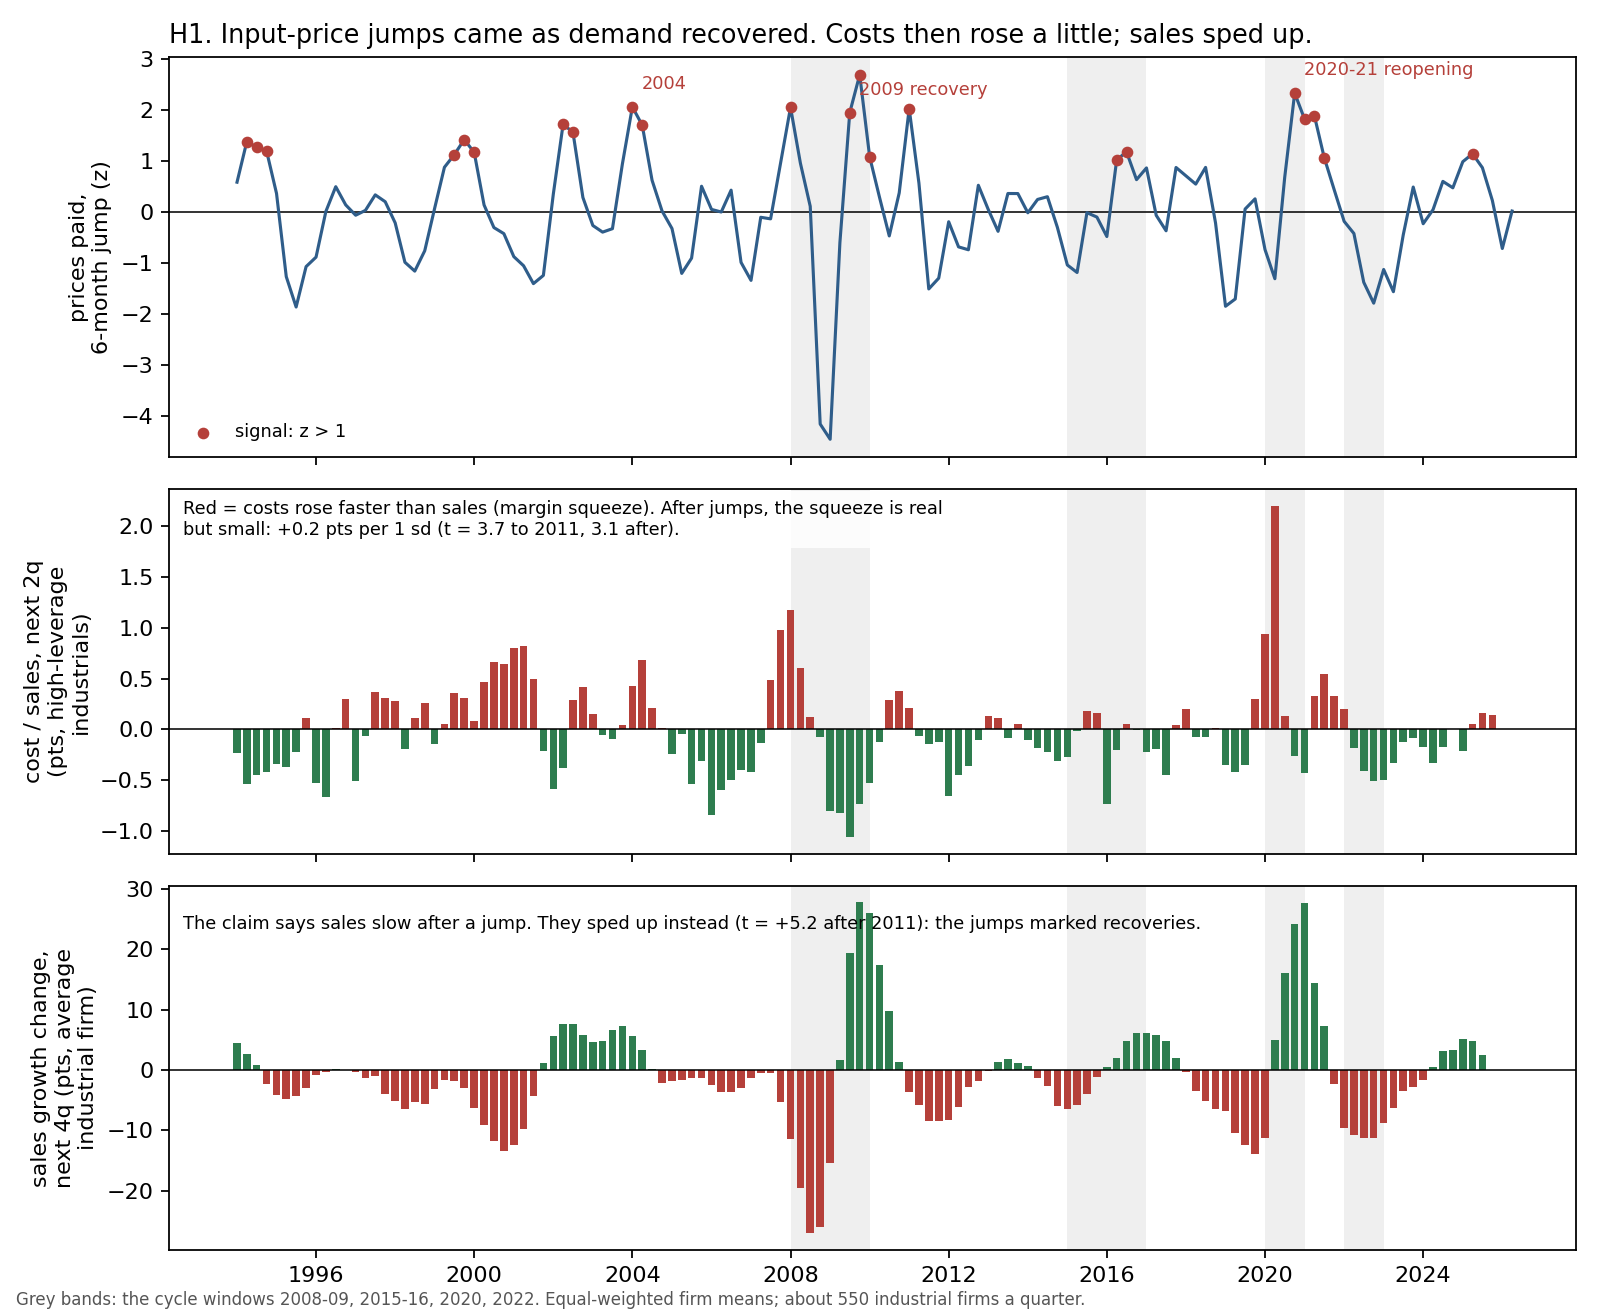
\includegraphics[width=0.93\linewidth]{figures/wt_h1_story.png}
\caption{Top: the 6-month jump in prices paid; red dots are signals. Middle: the cost ratio of high-leverage industrial companies over the next 2 quarters. Bottom: the change in sales growth of the average industrial company over the next 4 quarters. The jumps came as demand recovered (2004, 2009, 2020--21). Sales then sped up.}
\end{figure}
The notes read a jump in input prices as a coming squeeze. In the data, most jumps came at the start of a recovery. Demand pushed input prices and sales up together. The squeeze on costs was real, but small, and it showed mainly in high-leverage industrial companies.

\subsection*{Do company sensitivities persist? (test C)}
\begin{figure}[H]\centering
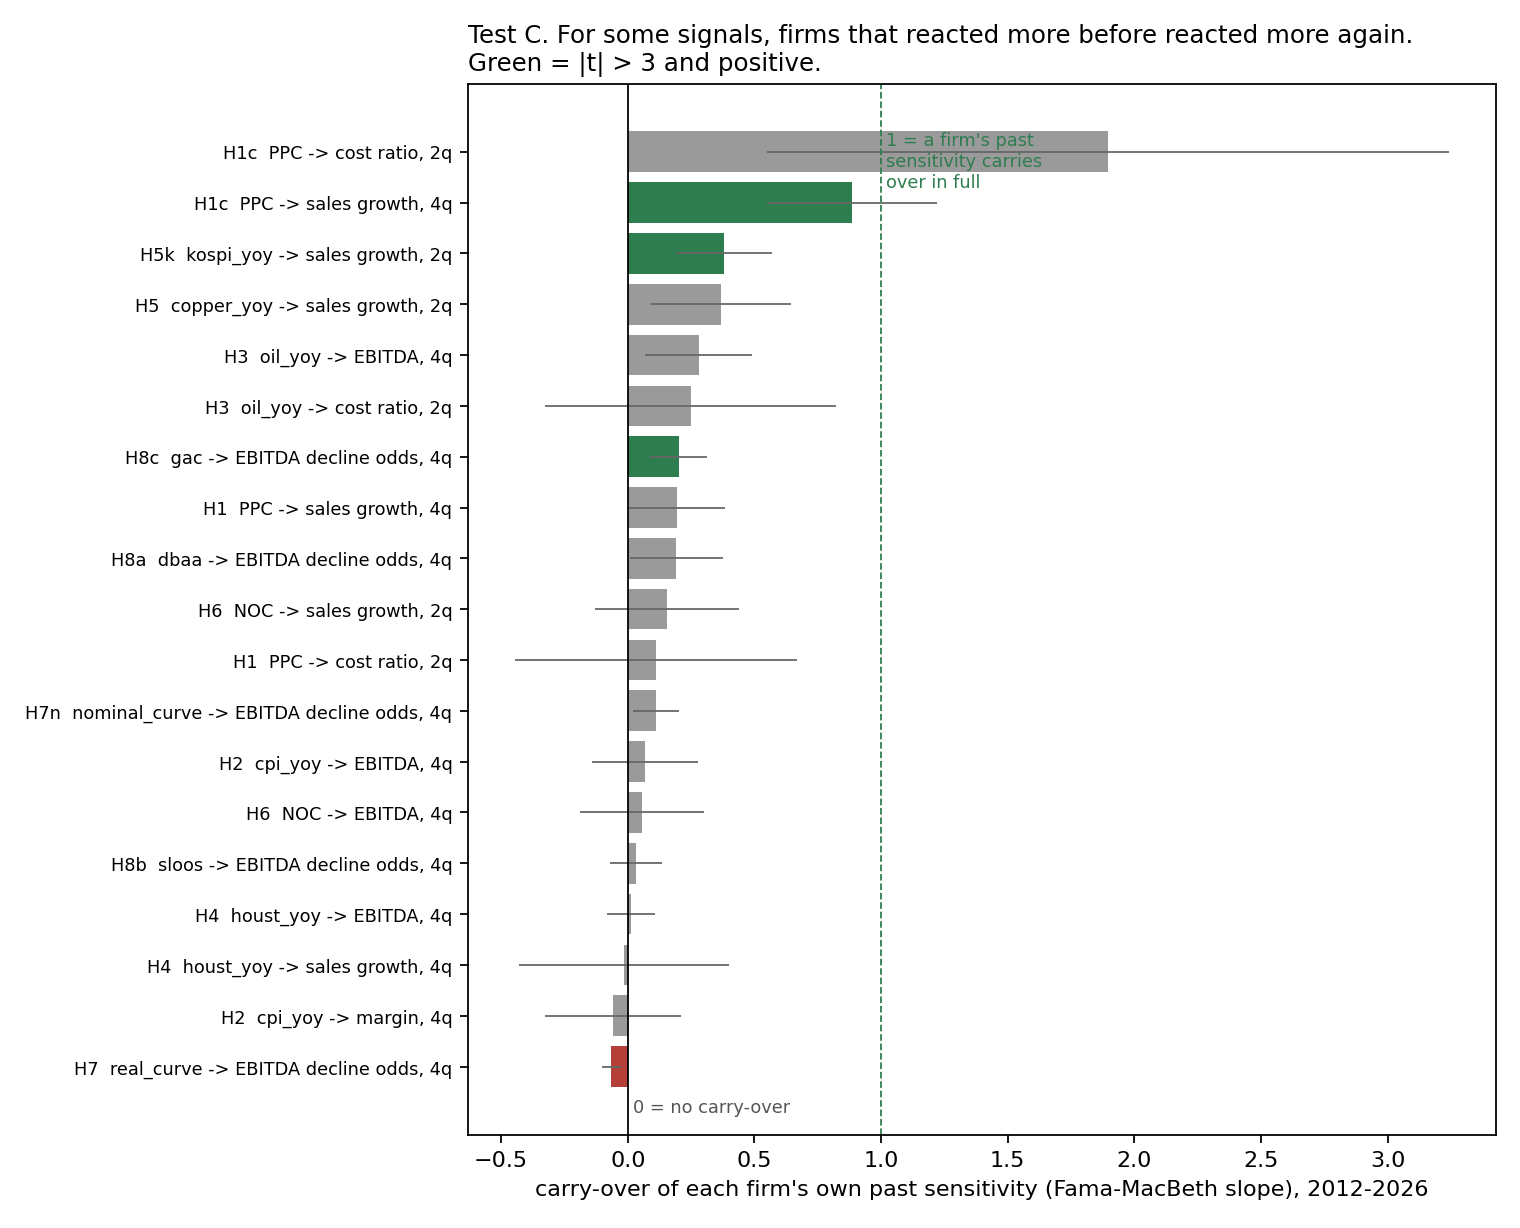
\includegraphics[width=0.85\linewidth]{figures/wt_exposure.png}
\caption{For each signal and outcome, the carry-over of each company's own past sensitivity, after 2011. Bars show $\pm 2$ standard errors.}
\end{figure}
For input-price jumps and sales (slope 0.89, $t$ 5.3), the Korean stock market and sales (0.38, $t$ 4.0), and factory activity and EBITDA declines (0.20, $t$ 3.6), companies that reacted more before reacted more again. For most other signals the carry-over is near zero.


\section{Robustness checks (added 24 October 2026)}\label{sec:robust}
A second agent stress-tested the 12 results that passed or came close (\code{scripts/wt\_robustness.py}). \textbf{Verdict: none is robust. Seven are fragile and five fail.}
\begin{enumerate}
\item \textbf{Placebo signals.} The agent replaced each signal with shifted and resampled copies that keep its autocorrelation. Under these placebos, one test falsely passes the full rule in 0.3\% of draws. At least one of the 92 tests passes in 18.7\% of draws. Three or more pass in 2.2\% of draws, against our 3 real passes. But two of the three use the same signal on the same companies.
\item \textbf{Correction for 92 tests.} Romano--Wolf and Benjamini--Yekutieli keep only H1c. Benjamini--Hochberg keeps 3.
\item \textbf{Few-quarter inference.} With equal-weighted cosine errors (Lazarus, Lewis, Stock, Watson 2018), the holdout $t$ of H1c falls from 3.05 to 2.22. The bar for $p < 0.05/8$ with about 54 quarters is about 3.8.
\item \textbf{Researcher choices.} Over 96 combinations of leverage cut-off, size floor, trimming, signal form, and weighting, H1c holds the claimed sign in 69\%. It is significant in 23\% ($|t| > 2$ after 2011 and Clark--West $p < 0.05$). With sales weights it disappears.
\item \textbf{A look-ahead fix.} The cycle check used the full-sample mean. The fix changes no pass flag.
\end{enumerate}

\section{The model's own macro inputs on high-yield issuers (tests S1--S4)}
A third agent ran the review tests of \code{docs/decisions/2026-10-24-review-sloos-pmi.md} on 16,906 issuer-quarters of 1,430 TRACE high-yield issuers, 2008--2026. Bank lending standards (S1), the factory survey as a level or by cyclical class (S2), and each phase vote (S3) failed the out-of-sample log-score rule. Leaving out 2020 (S4) did not rescue lending standards. After 2009, the full macro vector did not beat a model that uses the sector alone. The same agent found a defect: \code{hy/sources/trace\_panel.leverage\_as\_of} can sum four quarters that are not consecutive when a quarter is missing.

\section{What it means for the model}
\begin{enumerate}
\item \textbf{Add no Wolfe Trahan series to the forecast inputs $m_t$ of the downside model.} None improves the forecast of company results reliably. The two passes are small (H1c) or borderline (H5k).
\item \textbf{Use the confirmed directions in the stress scenarios.} In an inflation path, lower consumer EBITDA and margins (H2). In an oil path, raise energy EBITDA and consumer costs (H3). These are signs from history, not forecasts.
\item \textbf{Review the model's own macro inputs.} After 2011, bank lending standards and the factory survey did not predict company EBITDA declines. The Baa spread did a little. The downside model (methodology 5.2) uses all three. Open a decision page and rerun this test on the issuer universe before the model relies on them.
\item \textbf{Estimate sensitivity per issuer where it persists.} For input prices and global demand, past company sensitivity carries over. A sensitivity per issuer, shrunk toward its sector, may beat one sensitivity per sector (the current \code{fit\_sector\_beta}). Test that before use.
\end{enumerate}

\section{Limits}
\begin{enumerate}
\item The company data is Compustat's current view, after restatements. It shows what happened, not what investors saw first.
\item Sales are in dollars, so inflation raises them. Cost ratios and margins do not have this bias.
\item Some groups are small: about 55 housing-linked and 40 auto companies a quarter. The high-leverage tests for these groups have too few companies after 2011.
\item The family has 92 tests; 87 have every statistic. Under the null, at least one of the 92 passes the full rule in 18.7\% of placebo draws (Section~\ref{sec:robust}).
\item GICS codes are today's. A company that changed sector counts in its current one.
\item The signal transforms follow the charts in the notes. H1c is a second transform of the same claim.
\end{enumerate}

\section*{Reproduce}
Results go to \code{data/raw/backtest/wt\_firm\_*.json}.
\begin{verbatim}
PYTHONPATH=. python3 scripts/wt_tests.py     # all claims
PYTHONPATH=. python3 scripts/wt_figures.py   # the figures
python3 -m pytest -q tests/test_wt_tests.py  # 12 tests
\end{verbatim}
Inputs: \code{data/raw/compustat/fundq\_nonfin.parquet} (WRDS, \code{comp.fundq}), \code{data/raw/macro/} (Philadelphia Fed survey, FRED). Vendor data stays out of git.

\end{document}
